% !TEX root = ../thesis.tex
\chapter{Syntetická časť}
\label{methodology}

V tejto časti chcem nielen opísať konečný produkt, ktorý som vytvoril, ale aj celú cestu jeho vývoja. Týmto spôsobom pomôžem čitateľom tejto práce, aby sa pri vývoji podobných vzdelávacích projektov nedopustili podobných chýb.
Vývoj celého projektu som rozdelil do nasledujúcich etáp: 
\begin{enumerate}
    \item Vývoj meteorologickej stanice (1-2 vrstvy architektúry).
    \item Vývoj aplikácie (4. vrstva architektúry).
\end{enumerate}
Samostatnou etapou je testovanie celeho riešenia, ale to bude trochu neskôr.
\section{Počiatočný vývoj meteostanice}
Svoj vývoj som začal od prvých vrstiev podľa konceptu architektúry tohto projektu \ref{iot}, pretože je to pre mňa najlogickejšie riešenie. Preto som ako prvú vec začal vyvíjať meteorologickú stanicu.
\subsection{Prvé pokusy}
Keď som začal pripravovať projekt, nemal som jasný plán postupu ani predstavu o tom, ako by mala meteorologická stanica vyzerať vo svojej konečnej podobe. Kvôli nedostatku skúseností a praktických zručností som mal pri vypracovávaní projektu problémy. Prvé pokusy vývoja boli skôr experimentmi a oboznamovaním sa s výrobným procesom než serióznym vývojom. Po niekoľkých týždňoch takejto neefektívnej práce som však presne pochopil, ako tento projekt vyvíjať a aké základné funkcie musí tento projekt obsahovať. 

Veľmi dôležitú úlohu zohrala skutočnosť, že som pomerne intenzívne komunikoval so svojim veducim praci, ktorý mi v rámci možností radil vo všetkých otázkach, ktoré ma v súvislosti s procesom vivoja zaujímali.

Na začiatku vývoja projektu som používal \textit{Raspberry Pi Pico WH} a všetky pripojenia modulov som robil na \textit{breadboarde} (obr. \ref{breadboard}). Ale po čase som na uľahčenie vývoja začal používať \textit{Cytron Maker Pi Pico Base}.

\begin{figure}[!ht]
    \centering
    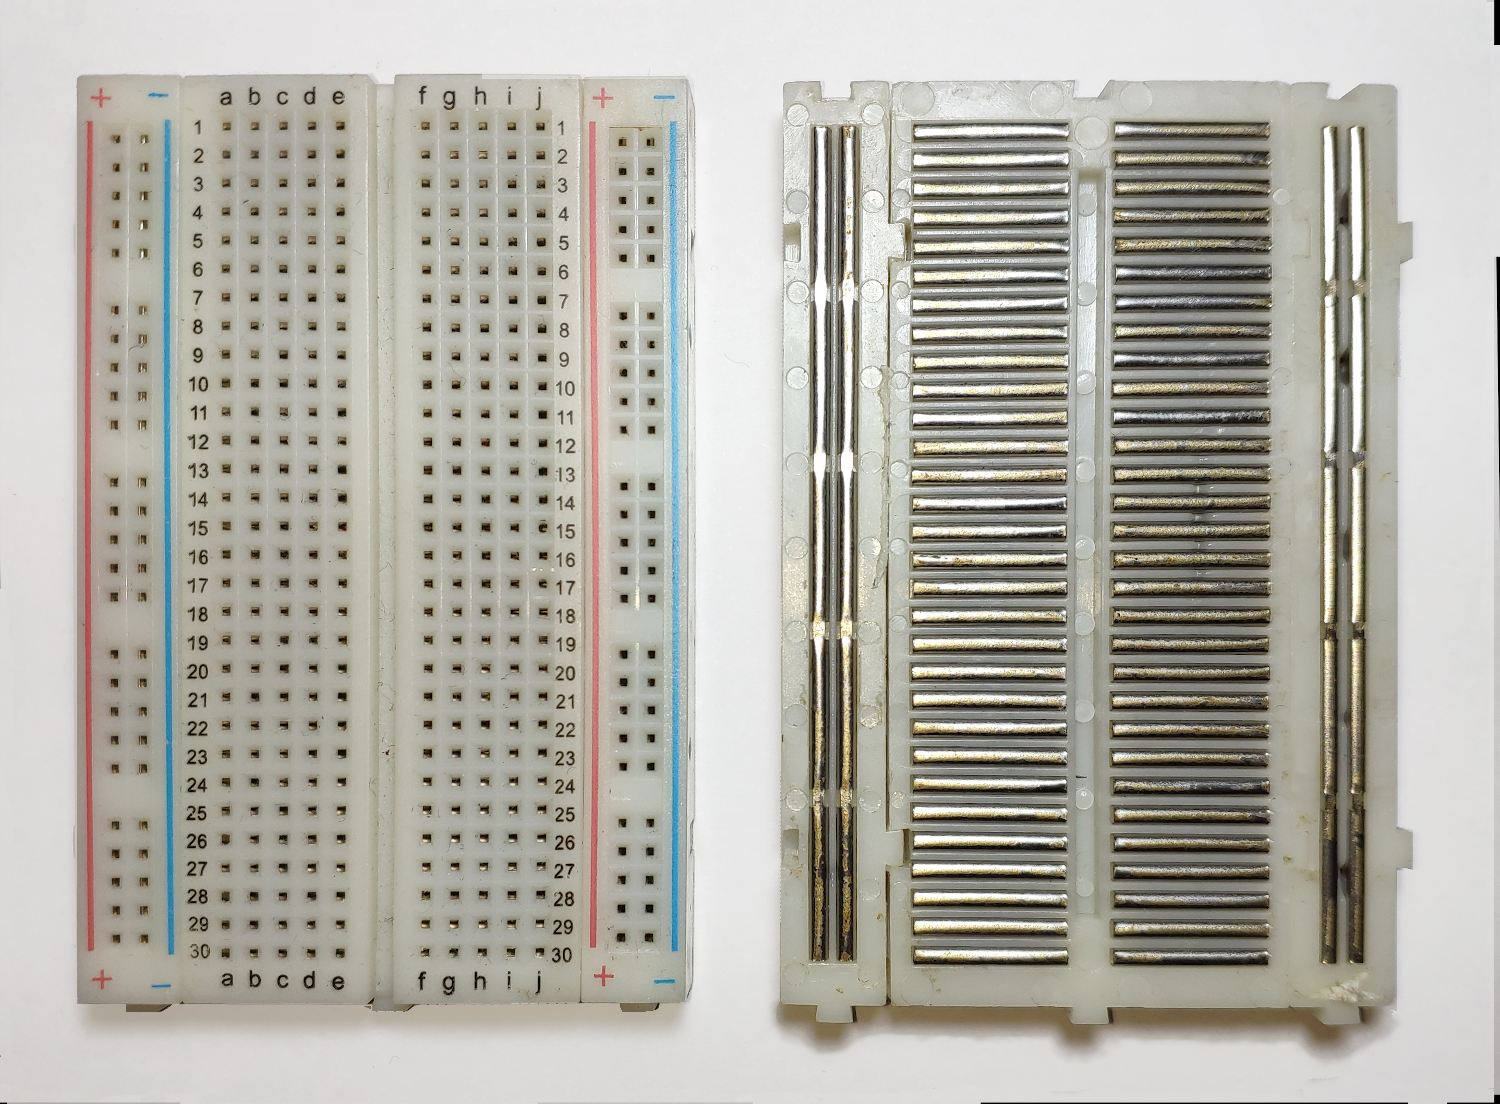
\includegraphics[width=\textwidth]{figures/breadboard}
    \caption{Vzhľad breadboardu z oboch strán\label{breadboard}\cite{breadboard}}
\end{figure}

\subsection{Zásady vývoja}
Pre správne splnenie úloh, musel som si vytvoriť podrobný, postupný plán činnosti pre vývoj meteostanice. 

Po premyslení tohto problému som prišiel s nasledujúcim akčným plánom:
\begin{enumerate}
    \item Vytvoriť hardvérovú časť meteostanice, konkrétne:
    \begin{itemize}
        \item Model toho, čo by mala táto meteorologická stanica obsahovať.
        \item Nakresliť elektricky obvod na pripojenie modulov.
        \item Vykonanie schémy na reálnom príklade.
    \end{itemize}
    \item Vytvoriť softvérovú časť meteorologickej stanice a implementovať nasledujúce funkcie:
    \begin{itemize}
        \item Zber údajov zo senzorov.
        \item Odosielanie údajov na \gls{mqtt} broker.
        \item Úspora energie (zabezpečiť možnosť autonómie).
        \item Tolerancia porúch.
        \item Dodatočné fičury.
    \end{itemize}
\end{enumerate}

%%------------------------------------------------------------------------

\section{Hardvérová časť meteostanice}
Meteorologická stanica by mala odčítať nasledujúce údaje: 
\begin{itemize}
    \item Teplota
    \item Vlhkosť vzduchu
    \item Intenzita svetla
\end{itemize}
Na tieto úlohy som použil senzor \gls{ldr} (intenzita svetla) a \gls{dht} (teplota a vlhkosť). Namiesto \gls{dht} by bolo možné použiť samostatné snímače teploty a vlhkosti, ale to je zbytočná komplikácia procesu vývoja. Namiesto \gls{dht} je môžne použiť novšiu verziu DHT22. V ich zapojení nie je osobitný rozdiel, ale na softvérovej úrovni novšia verzia používa inú knižnicu.

Počas priameho vývoja som sa stretol s problémom, že počas autonómnej prevádzky zariadenia nie je jasné, či funguje alebo má problém. Preto som do zariadenia pridal \gls{led} diódu, ktorá informuje vývojára o stave meteostanice.

Na pripojenie k \textit{Raspberry Pi Pico} budete potrebovať dva rezistory,
a to 10k$\Omega$
  a 220k$\Omega$.

  Konečný zoznam použitých komponentov je tu:
\begin{itemize}
    \item \gls{dht} 
    \item \gls{ldr}
    \item \gls{led} dióda
    \item 10k$\Omega$ rezistor
    \item 220k$
    \Omega$ rezistor
\end{itemize}
Na obrázku \label{schema} vidíme schému pripojenia všetkých modulov k doski \textit{Raspberry Pi Pico}. 

\subsection{Schéma zapojenia}
Ako už bolo opísané v teoretickej časti, projekt bude vyvinutý na základe doski \textit{Raspberry Pi Pico W}. Preto bola všetka práca vykonaná na tejto doske. Ale ja som otestoval fungovanie svojho projektu aj na \textit{ESP32} so zabudovaným WiFi modulom a môžem povedať, že som žiadne problémy nezistil. 

Preto sa v prípade potreby môže projekt realizovať aj pomocov doski na báze čipu \textit{ESP32}, a nie \textit{Raspberry Pi Pico W}. Chcem však upozorniť, že pred vedením kurzu musí učiteľ dôkladne otestovať verziu \textit{ESP32}, ktorú majú študenti k dispozícii, pretože existuje veľa konfigurácií dosiek s čipom \textit{ESP32} a ja nemôžem zabezpečiť fungovanie projektu na každej z nich. To znamená, že \textit{Raspberry Pi Pico W} je zárukou, že všetko bude fungovať tak, ako som ako vývojár zamýšľal. 

Ak sa teda vrátime k téme pripojenia jednotlivých modulov k doske mikroprocesora, potrebujeme dva digitálne piny na pripojenie diódy a \gls{dht} a jeden analógový pin na pripojenie \gls{ldr} senzora. Je potrebné poznamenať, že \gls{ldr} senzory sú dvoch typov, s digitálnymi a analógovými výstupmi. V projekte možno použiť obe verzie, ale je potrebné zohľadniť rozdiel v ich pripojení na softvérovej úrovni. Ja použijem analógovú verziu \gls{ldr}, pretože je súčasťou \textit{Arduino Kit}.

\begin{figure}[!ht]
    \centering
    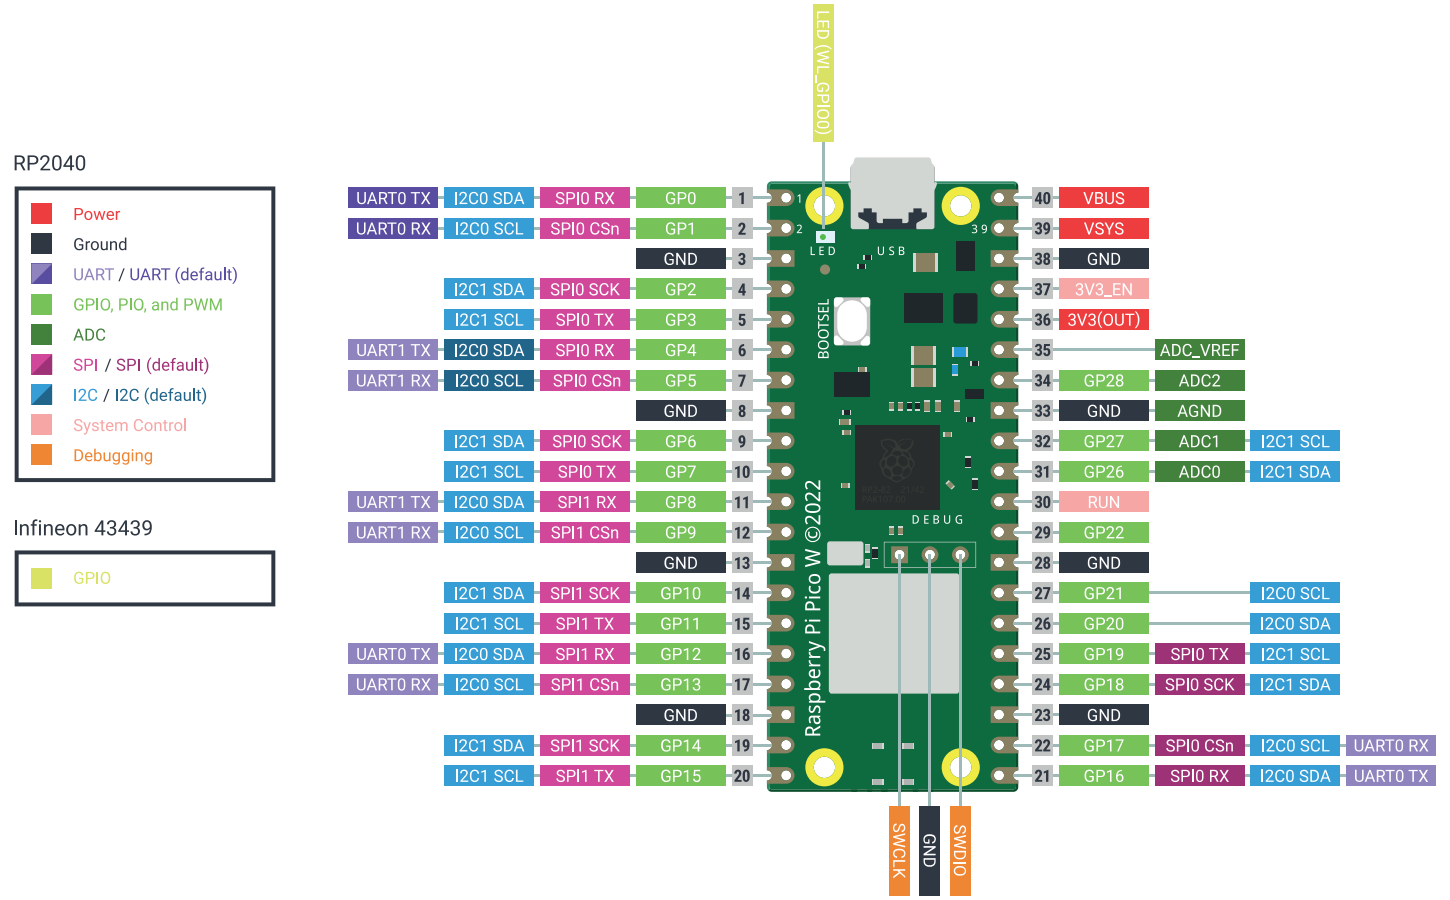
\includegraphics[width=\textwidth]{figures/raspberry_pi_pico}
    \caption{Rozloženie pinov na doske \textit{Raspberry pi pico W} \label{pico} \cite{piPico}}
\end{figure}

Ako vidne na obrázku \ref{pico}, \textit{Raspberry Pi Pico W} má iba tri analógové piny, a to: GP26, GP27, GP28. Môžete použiť ktorýkoľvek z nich, ja použijem GP26. Na pripojenie \gls{dht} a \gls{led} diódy môžete použiť ktorýkoľvek z dostupných digitálnych pinov, ja použijem GP21, a GP20. Na obrázku \ref{schema} môžete vidieť celú schému pripojenia k mikroprocesoru \textit{Raspberry Pi Pico W}. 

\begin{figure}[!ht]
    \centering
    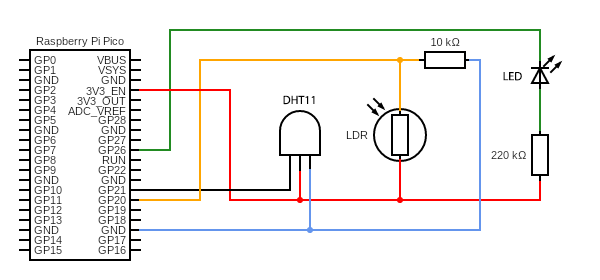
\includegraphics[width=\textwidth]{figures/circuit}
    \caption{Chéma pripojenia k doske Raspberry pi pico W \label{schema}}
\end{figure}

Dodatočne by som chcel upozorniť, že schéma zapojenia znázornená na obrázku \ref{schema} môže byť v niektorých prípadoch nefunkčná, pretože počet pinov na rôznych verziách modulov (napr. \gls{dht}) sa môže líšiť od toho, čo som uviedol. Preto by mal učiteľ pred vedením kurzu skontrolovať existujúcu konfiguráciu modulov a v prípade potreby zmeniť schému zapojenia.

\subsection{Príklady realizácie schémy zapojenia}
Celkovo som tento schému (obrázok\ref{schema}) realizoval v troch formách:
\begin{enumerate}
    \item Pomocou \textit{Raspberry Pi Pico W} (obrázok \ref{f_pico}).
    \item Pomocou \textit{Raspberry Pi Pico W} s použitím \textit{Cytron Maker Pi Pico Base W} (obrázok \ref{f_b_pico}).
    \item Pomocou \textit{ESP32} (obrázok \ref{f_esp32}). 
\end{enumerate}

Ako je môžne vidieť na obrázkoch \ref{f_pico} a \ref{f_esp32}, medzi vzhľadom pripojenia \textit{ESP32} a \textit{Raspberry Pi Pico W} nie je veľký rozdiel. Najjednoduchšie sa pripájal \textit{Raspberry Pi Pico W} s pomocnou doskou (obr. \ref{f_b_pico}), pretože nebolo potrebné použiť dodatočné rezistory ani veľké množstvo káblov.

Môžem tiež poznamenať, že schéma rozpojenia na obrázku \ref{schema} je len príkladom a ak spojenie urobíte trochu inak pri dodržiavaní logiky spojenia, nemali by vzniknúť žiadne problémy.

Pri práci s mikroprocesormi je dôležité dodržiavať bezpečnostné pravidlá, konkrétne zabrániť skratom pri zostavovaní fyzickej kópie projektu. Pri práci s ESP32 som kvôli nedostatku skúseností spálil mikroprocesor skratom. Viac takýchto incidentov som už nepripustil.

\begin{figure}[!ht]
    \centering
    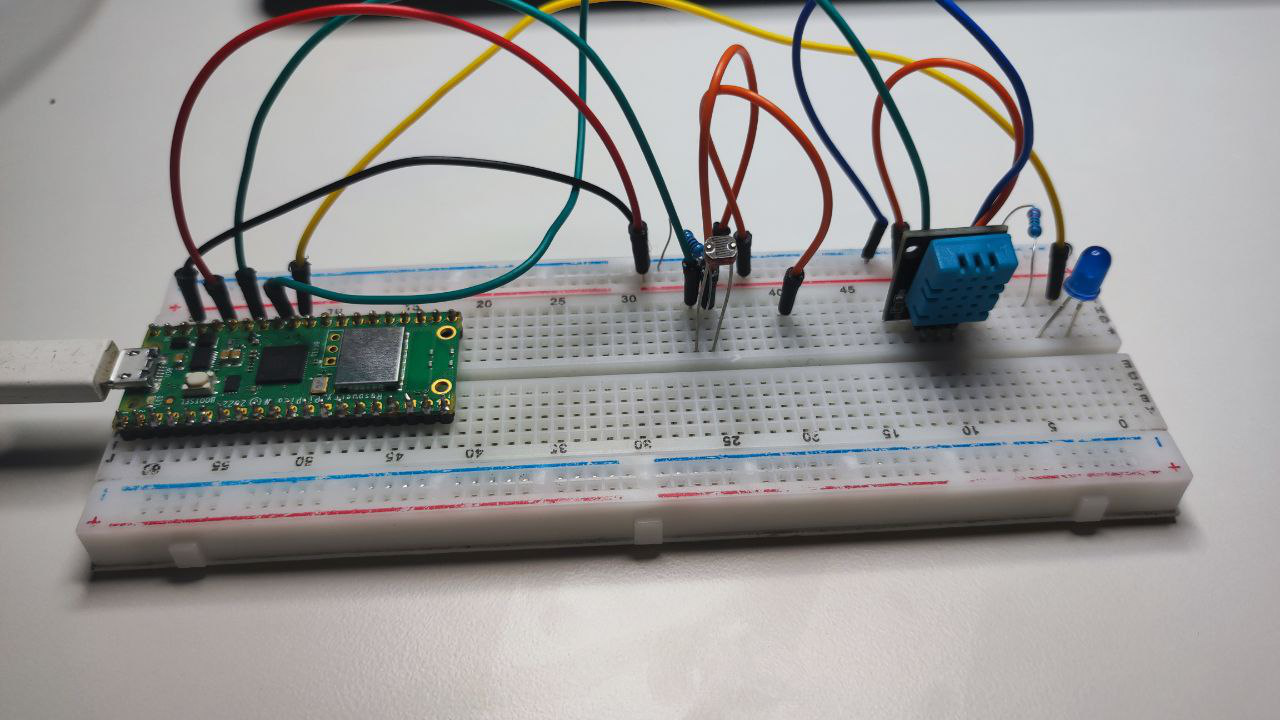
\includegraphics[width=\textwidth]{figures/f_pico}
    \caption{Fyzický príklad schémy zapojenia \ref{schema} pomocou \textit{Raspberry Pi Pico W} \label{f_pico}}
\end{figure}

\begin{figure}[!ht]
    \centering
    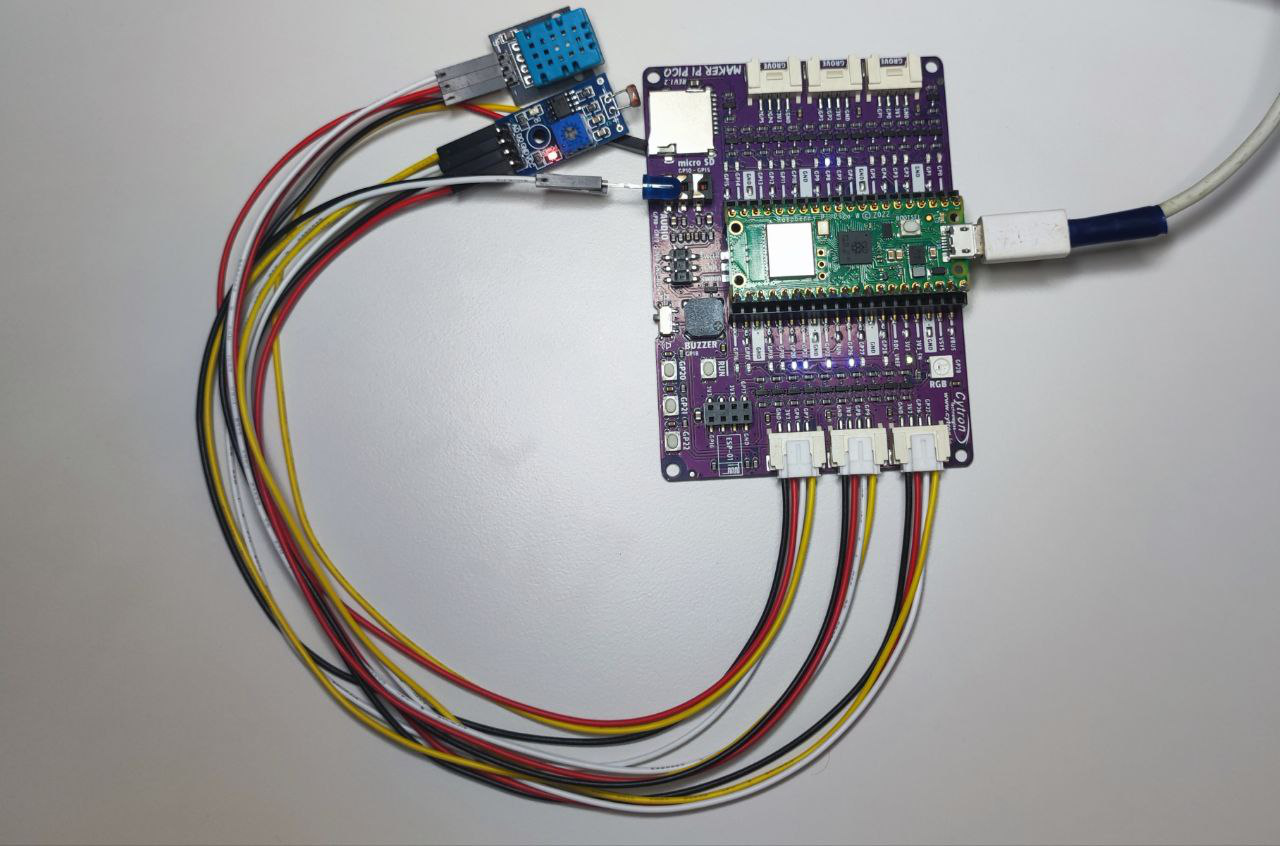
\includegraphics[width=\textwidth]{figures/f_bord_pico}
    \caption{Fyzický príklad schémy zapojenia \ref{schema} pomocou \textit{Raspberry Pi Pico W} s doplnkovou doskou \textit{Cytron Maker Pi Pico Base}\label{f_b_pico}}
\end{figure}

\begin{figure}[!ht]
    \centering
    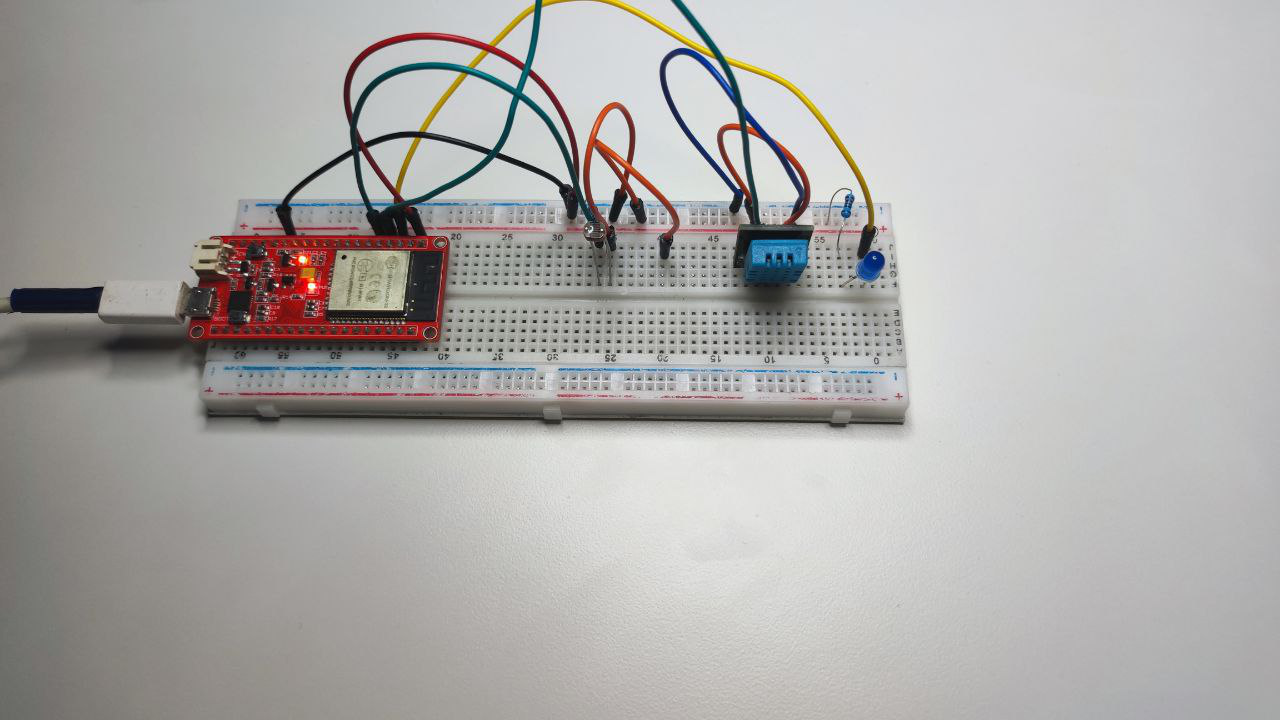
\includegraphics[width=\textwidth]{figures/f_esp32}
    \caption{Fyzický príklad schémy zapojenia \ref{schema} pomocou \textit{ESP32} \label{f_esp32}}
\end{figure}

%%------------------------------------------------------------------------

\section{Vývoj softvérovej časti meteostanice}
Softvér bol napísaný v programovacom jazyku \textit{MicroPython}, ako bolo napísané v predchádzajúcich častiach bakalárskej práce. 

Softvér pre meteorologickú stanicu bol vyvinutý v troch iteráciách:
\begin{enumerate}
    \item Počiatočné vytvorenie kódu so všetkými potrebnými funkciami.
    \item Refaktoring.
    \item Testovanie.
\end{enumerate}
V nasledujúcich podkapitolách podrobnejšie opíšem každú z týchto fáz.

\section{Hlavná časť vývoja (Prvá iterácia)}
\subsection{Postup vývoja}
V prvej iterácii vývoja kódu som sa nestaral o čistotu kódu a nerobil som žiadny refaktoring. To mi umožnilo sústrediť sa na samotný vývoj. 

Počas vývoja kódu som postupne pridával nové funkcie do meteorologickej stanice a snažil som sa dodržať vyššie uvedený plán vývoja. 

Pozrime sa na celý vývojový cyklus prvej iterácie a podrobnejšie rozoberme jednotlivé fázy pridávania nových funkcií pri zachovaní časovej hierarchie pridávania do projektu:
\begin{enumerate}
    \item \textit{Čítanie senzorovych dát} - implementoval som možnosť čítať metriky vlhkosti, teploty a svetla zo senzora \gls{ldr} a \gls{dht}. 
    
    Aby som zabránil načítaniu nesprávnych informácií, odčítam údaje 3-krát a vypočítam z nich medián. Ak sa teda z nejakého neznámeho dôvodu jedenkrát odčítajú nesprávne údaje, v nasledujúcich krokoch sa nezohľadnia.
    
    \item \textit{Pripojenie k internetu} - táto fáza bola najjednoduchšia na realizáciu.
    \item \textit{Pripojenie k \gls{mqtt}} - na implementáciu tejto a ďalšej etapy som použil knižnicu tretej strany, pretože základný balík \textit{Micropythonu} neobsahoval knižnicu, ktorú som potreboval. 
    \item \textit{Odoslanie údajov} - zozbierané a spracované údaje z prveho kroku sa odošlú do sprostredkovateľa \gls{mqtt}. 
    
    V počiatočných fázach som údaje posielal vo forme troch čísel, ale časom som si uvedomil, že tento typ údajov sa dosť ťažko číta, preto som začal údaje posielať vo forme \gls{json} správy.
    \item \textit{Šetrenie energie} - keďže meteorologická stanica má byť autonómna, šetrenie energie je dôležitou súčasťou tohto produktu. 
    
    Šetrenie energie som realizoval znížením taktu procesora, alebo takzvaným \textit{uspávaním} mikroprocesora. Dosahuje sa to pomocou špeciálnych príkazov a v prvých fázach vývoja som používal funkciu \verb|sleep()|, ktorá pozastaví aktuálny proces, čím sa zníži zaťaženie procesora. V budúcnosti som ju však nahradil energeticky úspornejšou funkciou \verb|deepsleep()|, ktorá zastaví všetky aktuálne procesy a prejde do úsporného režimu. 
    
    Túto fázu som vyvinul na základe týchto uvedených experimentov\cite{spotrebaEnergie1}\cite{spotrebaEnergie2}\cite{spotrebaEnergie3}.
    \item \textit{Problémová signalizácia} - ak meteorologická stanica nie je pripojená k počítaču, spotrebiteľ alebo vývojár nemá možnosť zistiť aktuálny stav systému bez prístupu k sériovému portu. Preto som sa v tomto bode rozhodol pridať \gls{led} diódu, ktorá bude signalizovať aktuálny stav zariadenia. 
    
    Teraz počas prevádzky zariadenia dióda signalizuje úspešnosť takých akcií, ako napr: 
    \begin{itemize}
        \item Pripojenie k wifi. 
        \item Pripojenie k sprostredkovateľovi \gls{mqtt}.
        \item Odosielanie údajov.
    \end{itemize}
    
    Ak dióda svieti 5 sekúnd, akcia bola úspešná, a ak bliká, akcia sa nepodarila. Na lepšie označenie problémov možno čas blikania a ich počet pre jednotlivé akcie meniť. 
    \item \textit{Tolerancia porúch} - počas prevádzky meteostanice existuje možnosť, že pripojenie k internetu alebo k serveru \gls{mqtt} sa môže z nejakých príčin prerušiť. 
    
    V čase takýchto problémov s pripojením môže dôjsť k strate zozbieraných údajov, pretože sa nebudú môcť dostať na server. Preto som sa rozhodol tento problém vyriešiť nasledujúcim spôsobom. 
    
    Pred odoslaním údajov sprostredkovateľovi \gls{mqtt} program skontroluje sieťové pripojenie a ak nie je dostupné, uloží zozbierané údaje do buffer súboru. Ak sa internetové pripojenie počas nasledujúcich iterácií opäť objaví, všetky údaje, ktoré sa nahromadili v súbore, sa odošlú na server. Toto je pomerne jednoduchý, ale účinný algoritmus.
    \item \textit{Aktualizácia času} - pri vývoji predchádzajúceho kroku som narazil na problém, že odoslané údaje sa nedajú rozlíšiť podľa času ich načítania. To znamená, že strana servera nerozumie presnému času merania a potenciálny spotrebiteľ môže analyzovať údaje len podľa času ich odoslania na server. 
    
    Preto som do \gls{json} správy, ktorá sa posiela na server, pridal parameter \verb|time|, ktorý znamená presný čas tohto merania v UTC.  Narazil som však na ďalší problém. Konkrétne na problém kontextualizácie času. 
    
    Ak je aplikácia spustená cez \gls{ide}(napr. \textit{Thonny}), tak by nemal nastať žiadny problém, pretože \gls{ide} automaticky aktualizuje čas na mikroprocesore, ale ak je aplikácia spustená bez mikroprocesora, tak sa čas neaktualizuje a nastaví sa na začiatok éry\footnote{\textit{https://docs.micropython.org/en/latest/library/time.html}}(1970-01-01 00:00:00 UTC). Preto som do programu implementoval automatickú aktualizáciu času, ale na jej vykonanie je potrebné mať prístup na internet. 
\end{enumerate}
\subsection{Pomocná knižnica}
Pri vývoji softvéru pre meteorologickú stanicu ma napadlo vytvoriť samostatnú knižnicu s funkciami, o ktorých predpokladám, že by mohli byť pre študentov s malými skúsenosťami s programovaním dosť náročné. Mohla by tiež obsahovať niektoré funkcie, ktoré štandardizujú údaje.

Vytvoril som teda takúto knižnicu a pomenoval som ju \verb|helper.py|.

Táto knižnica obsahuje nasledujúce funkcie:
\begin{itemize}
    \item \verb|def do_connect_wifi(ssid, password)| - Pripája sa k zadanej sieti WiFi. \\Vráti: \verb|True|, \verb|False|.(v závislosti od úspešnosti pripojenia)
    \item \verb|def do_connect_broker(name, server, port, login, password)| - Pripája k \gls{mqtt} brokeru. \\Vráti: Objekt \gls{mqtt} brokera, \verb|None|.(v závislosti od úspešnosti pripojenia)
    \item \verb|def send_mqtt_mesage(mqtt, topic, mesage)| - Odošle správu na zadaný \gls{mqtt} broker. \\Vráti:  \verb|True|, \verb|False|.(v závislosti od úspešnosti pripojenia)
    \item \verb|def create_json(time, temperature, humidity, light)| - Konvertuje zadané údaje do formatu \gls{json}. \\Vráti: \gls{json} v textovej forme. \\Tento príkaz slúži na štandardizáciu správ odosielaných na \gls{mqtt} server.
    \item \verb|def read_light(adc_pin)| - Meria osvetlenie z daného pinu. \\Vráti: Percent osvetlenia od 0 do 100. 
\end{itemize}

\subsection{Kritické problémy, s ktorými som sa stretol počas vývoja.}
Ako som už napísal, pri práci s mikroprocesormi je potrebné dodržiavať bezpečnostné opatrenia, aby ste predišli rôznym nepríjemným situáciám. Pri vývoji softvéru sa však vývojár môže dopustiť niektorých nezrejmých chýb, ktoré môžu viesť k úplnej strate kódu, alebo dokonca firmvéru. Počas svojej práce som sa s jedným takýmto problémom stretol a v tejto časti ho opíšem, aby prípadný čitateľ tejto práce neurobil podobnú chybu.

Dovoľte mi teda uviesť stručný prehľad tohto problému. Pri opise vývoja som v časti o šetrení energie písal o vhodnejšom použití funkcie \verb|deepsleep()| namiesto funkcie \verb|sleep()|. Počas aktívneho vývoja, keď má váš kód nejaké problémy, sa však pri použití funkcie \verb|deepsleep()| môže váš kód dostať do tzv. $"$dead loop$"$. Zvyčajne sa problémy s $"$dead loop$"$ riešia reštartovaním systému, ale nie v prípade funkcie \verb|deepsleep()|. Aby fungovala správne, hlavný súbor vašej aplikácie sa musí volať start.py, to znamená, že je to súbor, ktorý sa spustí pri každom zapnutí mikroprocesora. 

Riešením tohto problému je úplné prepísanie systému mikroprocesora. Možno existujú humánnejšie spôsoby riešenia tohto problému, ale v mojom prípade je to jediný spôsob, ktorý som mohol urobiť. 

Aby ste tomuto problému predišli, odporúčam vám používať funkciu deepsleep() až v záverečných fázach, keď ste si istí, že program pracuje správne. V počiatočných fázach vývoja vám odporúčam používať funkciu \verb|sleep()|.

\subsection{Výsledok vývoja a potreba refaktoringu.}
Takže keď som implementoval všetky potrebné funkcie a vyriešil som všetky problémy súvisiace s vývojom meteostanice, získal som produkt, ktorý cyklicky vykonáva tieto kroky:
\begin{itemize}
    \item Prebudí sa a pripojí sa k sieti.
    \item Sníma a odosiela údaje na server. 
    \item Zaspí na 5 minút.
\end{itemize}

Je to veľmi jednoduchý algoritmus, ale pre meteostanicu nepotrebuje nič viac. V tejto etape už teda projekt vyzerá viac-menej dobre, takže je čas premýšľať o tom, ako budú môcť študenti realizovať projekt.

Po zamyslení sa nad touto otázkou som dospel k záveru, že na to, aby študenti mohli pracovať efektívne, je potrebné vytvoriť kostru projektu, na základe ktorej budú študenti vykonávať ďalší vývoj. To znamená, že namiesto toho, aby študenti robili všetko od začiatku, budú mať základ projektu a zoznam funkcií, ktoré musia urobiť. Pri tejto metóde študenti strácajú pocit neurčitosti a nepochopenia, a tak sa kód študentov stáva štandardizovanejším, čo zlepšuje možnosť hodnotenia. 

Koreň projektu je logické vytvoriť na základe už hotového projektu, teda toho, čo som už urobil. Je tu však jeden problém, momentálne je môj kód pre meteorologickú stanicu veľmi hrubý a neprehľadný na čítanie. Preto som dospel k záveru, že softvér, ktorý som vytvoril, je potrebné refaktorovať.

%%------------------------------------------------------------------------

\section{Refaktoring (Druhá iterácia)}
Takže v čase, keď som začal refaktorovanie, vyzeral môj projekt takto: 
\begin{itemize}
    \item \verb|main.py| - tu sa nachádza hlavná časť kódu. 
    \item \verb|helper.py| - pomocná knižnica, o fungovaní ktorej som už písal.
\end{itemize}

Kód v súbore \verb|main.py| bol pred refaktorovaním veľmi neprehľadný a bolo veľmi ťažké identifikovať funkcie, ktoré by mohli byť súčasťou kostry projektu. Preto bolo rozhodnuté rozdeliť kód v tomto súbore na niekoľko častí.

Počas jednej z konzultácií mi učiteľ Miroslav Biňas vnukol myšlienku, že proces fungovania meteostanice možno reprezentovať ako konečný stavový automat a kód projektu možno rozdeliť do jednotlivých stavov projektu. Táto myšlienka sa mi zdala naozaj veľmi chytrá, preto som kód projektu zmapoval na tento model. V nasledujúcich kapitolách budem podrobnejšie hovoriť o tom, ako tento koncept vyzerá a aký bol konečný výsledok.

\subsection{Konečný stavový automat v projekte}
Konečný stavový automat je koncept, ktorý opisuje veci v zmysle jednotlivých stavov a počet týchto stavov je konečný\cite{KA}. V našom prípade použijem tento pojem na opis cyklickej logiky meteostanice v rámci jednotlivých stavov.

Analyzoval som logiku meteostanice a identifikoval som nasledujúce stavy:
\begin{itemize}
    \item Inicializácia - zariadenie sa pripojí k wifi a \gls{mqtt} brokeru.
    \item Meranie - zariadenie meria parametre teploty, vlhkosti a svetla.
    \item Odosielanie - zozbierané údaje sa spracujú a odošlú na server \gls{mqtt}.
    \item Uspanie - zariadenie prejde do energeticky efektívneho režimu na konštantný čas.
\end{itemize}
Všetky tieto stavy sa cyklicky striedajú jeden za druhým donekonečna. Na obrázku \ref{ksa} môžete vidieť, ako vyzerajú vo forme diagramu.
\begin{figure}[!ht]
    \centering
    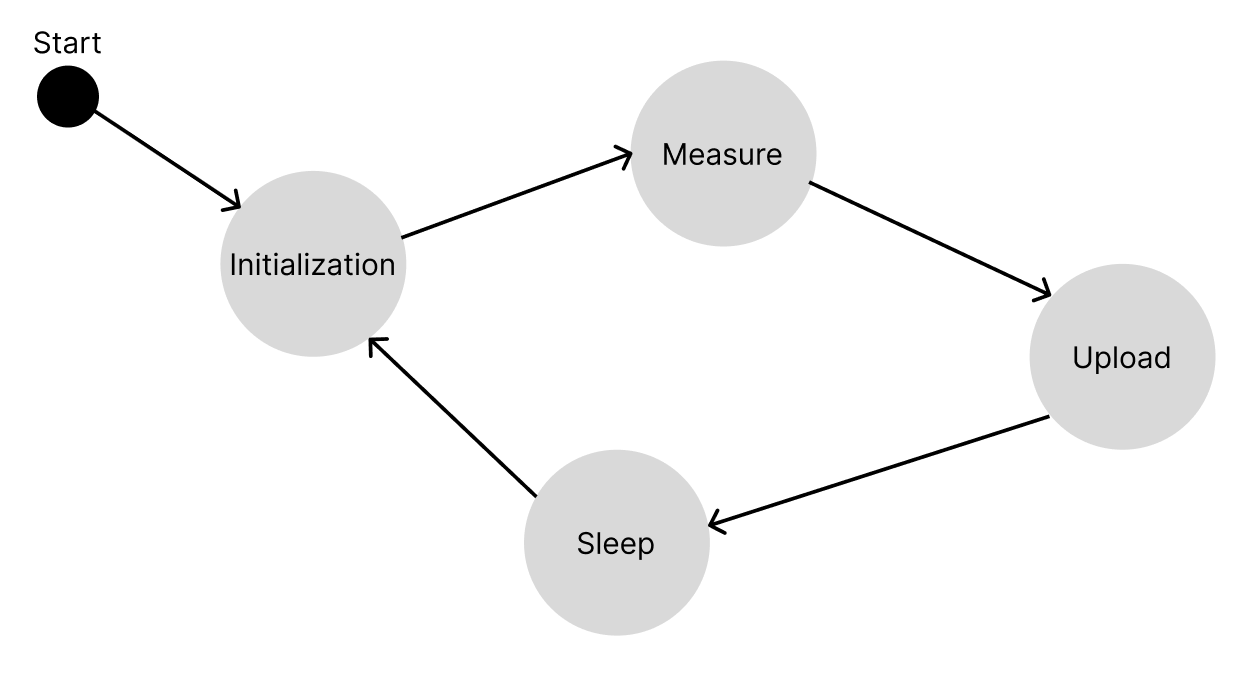
\includegraphics[width=\textwidth]{figures/KSA}
    \caption{Práca meteostanice vo forme konečno stavoho automatu. \label{ksa}}
\end{figure}

\subsection{Výsledok refaktorovania kódu.}
Takže na základe konečného stavového automatu zobrazeného na obrázku 1 som prepracoval štruktúru celého projektu. Nezmenený zostal len súbor \verb|helper.py|

Pre lepšie pochopenie novej štruktúry projektu najprv uvediem všetky súbory, ktoré sa v projekte nachádzajú: 
\begin{itemize}
    \item \verb|start.py| - štartovací súbor, ktorý obsahuje logiku prechodu z jedného stavu do druhého.
    \item \verb|states.py| - súbor, ktorý obsahuje celú logiku jednotlivých stavov.
    \item \verb|helper.py| - súbor s pomocnými funkciami.
    \item \verb|settings.py| - tu sa nachádzajú konštantné parametre, ktoré sa v projekte používajú na uľahčenie prístupu k nim.
\end{itemize}
Teraz sa pozrime na štruktúru projektu a jednotlivé súbory podrobnejšie.

Ako som povedal, poradie prechodu z jedného stavu do druhého sa nachádza v súbore \verb|start.py|, každý stav je obsiahnutý vo funkciách:
\begin{itemize}
    \item \verb|def init(context)| - inicializácia
    \item \verb|def measure(context)| - meranie
    \item \verb|def upload(context)| - nahrávanie
    \item \verb|def sleep_pico(context)| - uspávanie
\end{itemize}
Tieto funkcie sa nachádzajú v súbore \verb|states.py| a práve tieto funkcie budú musieť študenti naprogramovať. Okrem týchto funkcií môžu študenti vytvoriť aj iné funkcie, ale hlavné je, aby sa názov uvedených funkcií nemenil. Súbor \verb|start.py| obsahuje aj triedu \verb|Context|, ktorá sa používa ako globálna štruktúra s premennými. Tieto premenné sú pomocné a používajú sa v rôznych funkciách. Funkcie v súbore \verb|helper.py| nebudú študenti programovať a používajú sa skôr ako knižnicu. Súbor \verb|settings.py| obsahuje konfiguračné premenné, ktoré sa zvyčajne používajú len raz. Tieto premenné som oddelil do samostatného súboru, aby som zlepšil čistotu kódu a uľahčil zmenu týchto údajov.
%%------------------------------------------------------------------------

\section{Testovanie (Tretia iterácia)}
\subsection{Ciele}
Účelom testovania je skontrolovať, či projekt neobsahuje výrazné problémy alebo nejasnosti v návrhu projektu. Testovanie by sa malo vykonávať na cieľovej skupine projektu a malo by sa prednostne vzťahovať na celý projekt.

Ďalším účelom testovania je overenie množstva práce, ktorú študenti dokážu vykonať v stanovenom čase. Robí sa to preto, aby sa projekt dal ľahšie rozdeliť na niekoľko častí (prednášok). Je to preto, aby sa projekt ľahšie implementoval do kurzu.
\subsection{Príprava}
Test sa mal uskutočniť v Gymnáziume svätého Tomáša Akvinského\footnote{\textit{https://www.gta.sk/}}. Na test bola určená 1 hodina a 30 minút. Vo vymedzenom čase som chcel študentom odovzdať čo najviac informácií, preto som si pripravil podrobný plán postupu, aby sa minimalizovali časové straty.

Test som rozdelil na teoretickú a praktickú časť. V teoretickej časti som si dal za úlohu povedať o týchto veciach:
\begin{enumerate}
    \item Čo je to \gls{iot}.
    \item Porozprávať o vrstvách architektúry \gls{iot} riešení.
    \item Vysvetliť architektúru môjho projektu.
    \item Vyjadriť študentom, čo budú robiť v praktickej časti.
\end{enumerate}

Pri plánovaní praktickej časti som nemohol predpovedať, koľko práce budú študenti schopní urobiť v čase určenom na test. Preto som naplánoval pomerne veľa položiek, a to:

\begin{enumerate}
    \item Poskladanie hardvérovej časti projektu.
    \item Testovanie blikaním \textit{\gls{led}} diódy.
    \item Meranie hodnôt zo senzorov.
    \item Pripojenie k internetu a \gls{mqtt} brokeru.
    \item Odosielanie údajov vo formáte \gls{json}.
    \item Implementácia zníženia spotreby energie.
    \item Signalizácia problémov pomocou \textit{\gls{led}} diódy.
    \item Zápis a čítanie údajov zo súboru.
\end{enumerate}

Praktická časť bola implementovaná na doskách \textit{ESP32}, pretože škola mala k dispozícii len ich. S ohľadom na to som upravil schému pripojenia k doske. 

Na programovanie som sa rozhodol použiť \textit{\gls{ide} Thoony}, pretože už bolo nainštalované na školských počítačoch.

Pri príprave a realizácii testu mi pomáhal Šimon Pavlišin a ja som bol vedúcim testu.

\subsection{Úroveň znalostí študentov}

Test bol realizovaný na študentoch tretieho ročníka Gymnázia svätého Tomáša Akvinského. V čase testovania študenti už mali za sebou praktické úlohy s \textit{Arduino Uno} a \textit{ESP32}. Mali teda základné zručnosti v programovaní mikroelektroniky. Takéto schopnosti mohli zrýchliť niektoré fázy praktickej časti (napr. pripojenie modulov k doske \textit{ESP32}).

\subsection{Výsledky}

Na teste sa zúčastnilo 12 študentov s rôznou úrovňou motivácie a znalostí. Počas testu sa mi podarilo spracovať celú teoretickú časť a prvé dva body praktickej časti.  Študenti mali problémy s poskladaním hardvéru a mali veľké problémy s pochopením \textit{Thonny}, takže veľa času sme venovali riešeniu problémov súvisiacich s týmto \gls{ide}.

Podľa študentov bola teoretická časť pomerne ľahko pochopiteľná, ale praktická časť bola dosť nejasná.

\subsection{Záver}

Tento test umožnil získať veľa užitočných informácií a pomohol vyhnúť sa niektorým problémom pri písaní scenára pre lekcie. 

Fakt toho, že títo študenti už mali hodiny s \textit{ESP32}, im nedal výraznú výhodu, pretože moduly k \textit{EP32} pripojovali dosť dlho. Prekvapilo ma množstvo času stráveného riešením kritických problémov s \textit{\gls{ide} Thonny}. Študenti nechápali, ako ho používať, a robili veľmi jednoduché chyby, ale ich riešenie mi zabralo dosť času. Myslím si, že tento problém vznikol v dôsledku môjho zlého plánovania, pretože som predpokladal, že táto fáza nezaberie veľa času, a tak som jej nevenoval dostatočnú pozornosť. Túto skúsenosť zohľadním pri príprave svojich hodín.

Vo všeobecnosti mi tento test poskytol predstavu o približnom množstve informácií, ktoré musím poskytnúť na jednej vyučovacej hodine môjho kurzu. Poskytol mi tiež neoceniteľné skúsenosti pri práci so študentmi.

\section{Zhromažďovanie údajov na bráne a ich spracovanie}

Po ukončení vývoja meteorologickej stanice považujem za účelné ukázať študentom, ako pracovať so získanými údajmi, spracovať ich a vizualizovať. 

Ako už bolo popísané v teoretickej časti, najlepšie sa to robí pomocou programovacieho jazyka \textit{Node Red} na pripravenej \gls{iot} bráne. Vytvoril som teda pomerne jednoduchý program (obr. \ref{node}) na vizualizáciu údajov získaných z meteorologickej stanice. Jeho vizualizáciu si môžete pozrieť na obrázku \ref{nodeVisual}.
\begin{figure}[!ht]
    \centering
    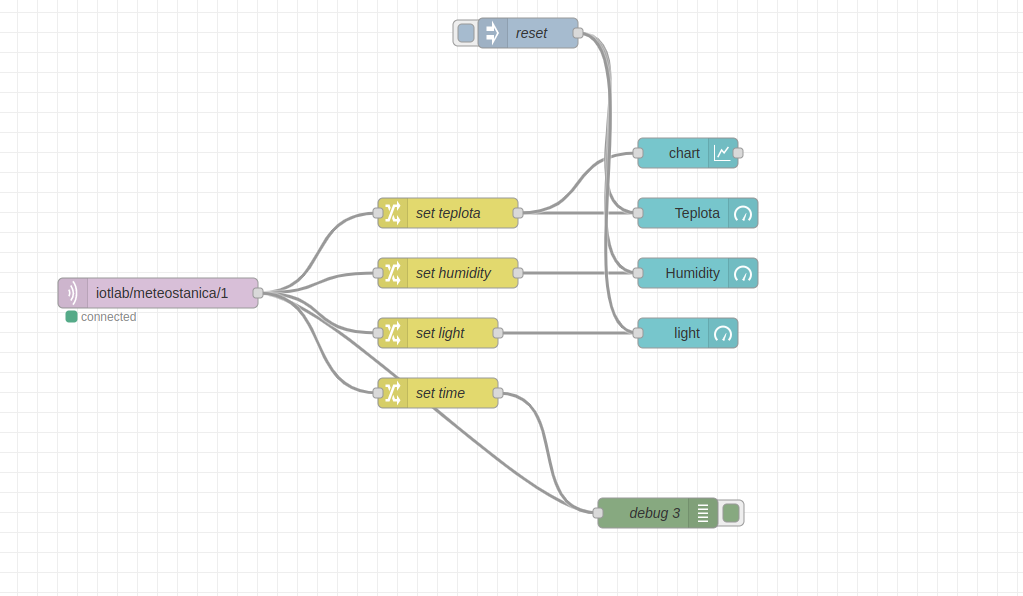
\includegraphics[width=\textwidth]{figures/node}
    \caption{Logika aplikácie na vizualizáciu dát vytvorenej v \textit{Node Red} \label{node}}
\end{figure}
\begin{figure}[!ht]
    \centering
    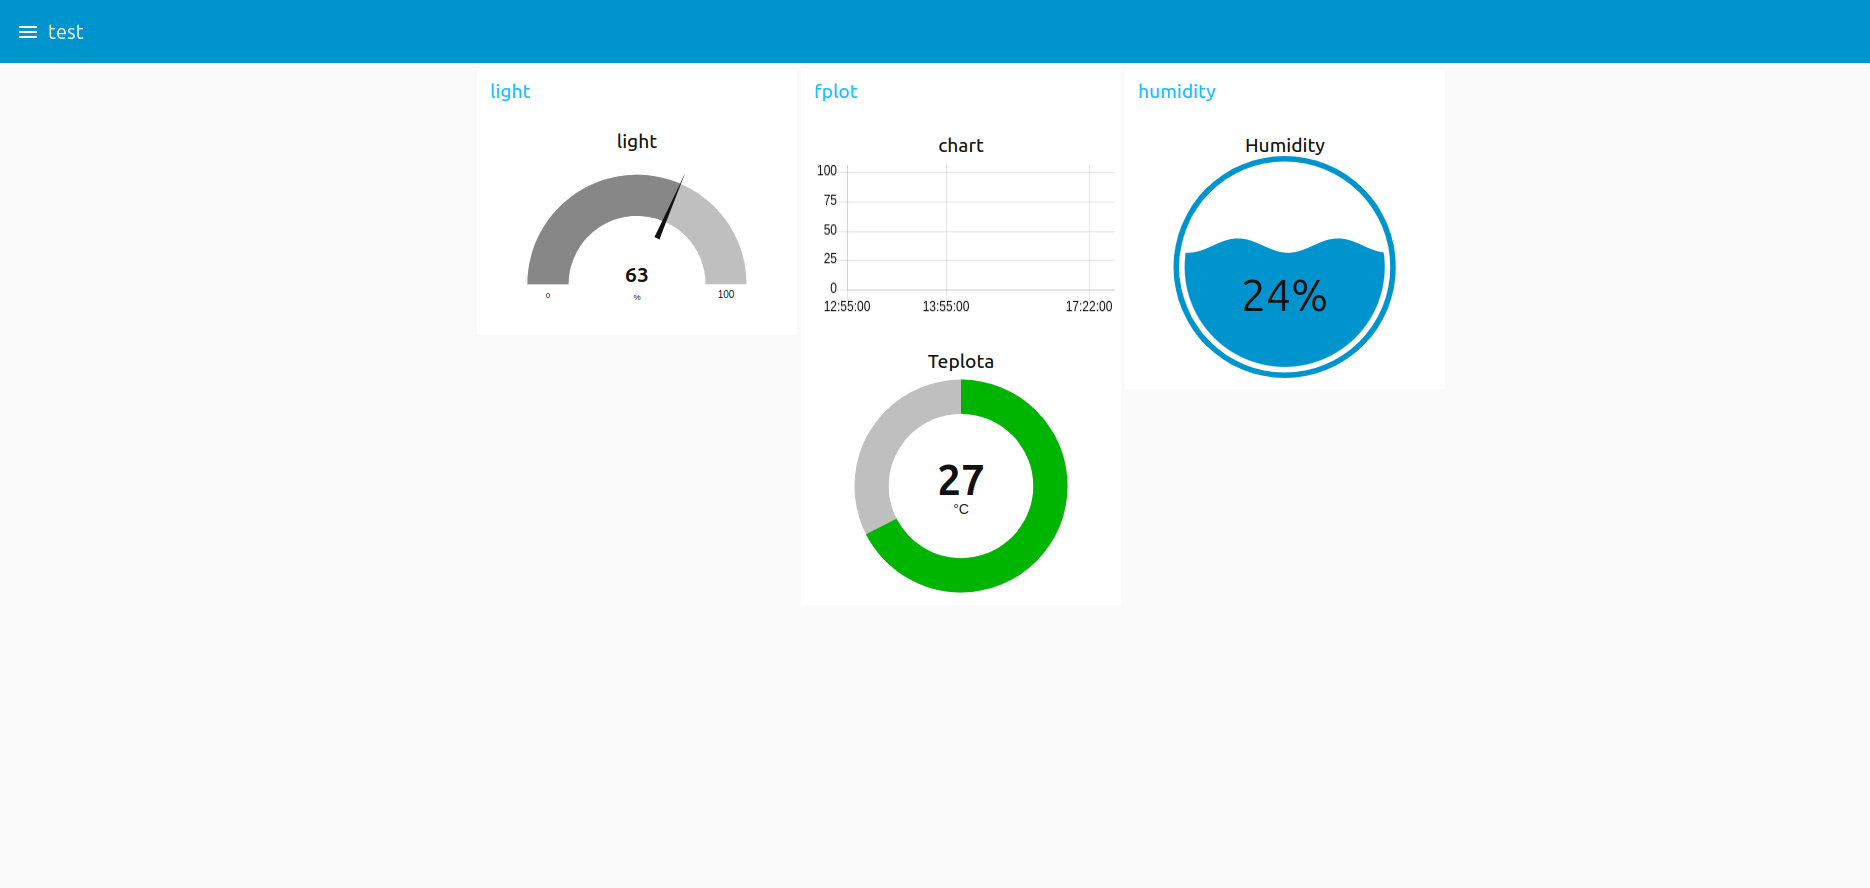
\includegraphics[width=\textwidth]{figures/node_obr}
    \caption{Vizualizácia aplikácie vytvorenej na \textit{Node Red}. \label{nodeVisual}}
\end{figure}
Napriek tomu, že logika programu je veľmi jednoduchá, na základe mojich skúseností môžem povedať, že na bežné zoznámenie s jazykom \textit{Node Red} tohto stačí. 

Program na obrázku \ref{node} je len príkladom. Učitelia si pri implementácii môjho projektu do svojho kurzu môže vytvoriť vlastný scenár na základe vedomostí svojich študentov.

\section{Analiza pridanej hodnoty projektu}
\subsection{Hlavná časť analýzy}
Táto časť opisuje cenu niekoľkých projektových konfigurácií, a konkrétne:
\begin{enumerate}
    \item Pomocou \textit{Raspberry Pi Pico WH} (obrázok \ref{f_pico}).
    \item Pomocou \textit{Raspberry Pi Pico WH} s použitím \textit{Cytron Maker Pi Pico Base W} (obrázok \ref{f_b_pico}).
    \item Pomocou \textit{ESP32} (obrázok \ref{f_esp32}). 
\end{enumerate}
Ceny som prebral z webovej stránky \textit{rpishop.cz}, pretože si myslím, že tam uvedené ceny plne zodpovedajú cenám na trhu. Okrem toho som analyzoval ceny na stránke \textit{aliexpress.com}, aby som zobraziť, potenciálne, najnižšie možné ceny. 

Treba poznamenať, že v čase písania tejto práce ešte neboli odstránené škodlivé následky krízy mikročipov\footnote{\textit{https://www.telefonica.com/en/communication-room/why-is-the-microchip-crisis-affecting-us-this-much/}}, takže cenová politika sa môže za nejaký čas výrazne zmeniť.  

Ako už bolo spomenuté v iných kapitolách, stredné školy na Slovensku už zvyčajne majú k dispozícii stavebnice Arduino Kit, ktoré obsahujú moduly potrebné na kurz: \gls{dht}, \gls{ldr}, \gls{led} diódy. Preto som sa rozhodol ich cenu do kalkulácie nezahŕňať. Pre \gls{gw} som sa rozhodol použiť \textit{Raspberry Pi 3 Model A+}, pretože tento model je dostatočne výkonný na svoje úlohy.

Všetky výpočty sú k dispozícii v tabuľkách \ref{tabESP32}, \ref{tabPico} a \ref{tabPicoDos}. Výpočty boli vykonané v mene Euro(\texteuro).

\begin{table}[!ht]
    \smallskip
    \centering
    \begin{tabular}{ | m{3cm} | m{2cm}| m{2cm} | m{2cm} | m{3cm} | } 
        \hline
         & \textit{ESP32} & \textit{Raspberry Pi 3 Model A+} & Celková cena & Cena projektu pre 30 študentov\\
        \hline
        rpishop.cz & 10,81 \texteuro & 33,88 \texteuro & 44,69 \texteuro & 358,18 \texteuro\\
        \hline
        aliexpress.com & 6,67 \texteuro & 85,43 \texteuro & 92,10 \texteuro & 285,53 \texteuro\\
        \hline
    \end{tabular}    
    \smallskip
    \caption{Analýza ceny projektu na základe dosky \textit{ESP32}. \label{tabESP32}}
\end{table}


\begin{table}[!ht]
    \smallskip
    \centering
    \begin{tabular}{ | m{3cm} | m{2cm} | m{2cm} | m{2cm} | m{3cm} | } 
        \hline
         & \textit{Raspberry Pi Pico WH} & \textit{Raspberry Pi 3 Model A+} & Celková cena & Cena projektu pre 30 študentov\\
        \hline
        rpishop.cz & 8,86 \texteuro & 33,88 \texteuro & 42,74 \texteuro & 308,54 \texteuro\\
        \hline
        aliexpress.com & 5,83 \texteuro & 85,43 \texteuro & 91,26 \texteuro & 260,33 \texteuro\\
        \hline
    \end{tabular}    
    \smallskip
    \caption{Analýza ceny projektu na základe dosky \textit{Raspberry Pi Pico WH}. \label{tabPico}}
\end{table}


\begin{table}[!ht]
    \smallskip
    \centering
    \begin{tabular}{ | m{7em} | m{4em} | m{4em} | m{2cm} | m{4em} | m{5em} | } 
        \hline
         & \textit{Raspberry Pi Pico WH} & \textit{Cytron Maker Pi Pico Base W} & \textit{Raspberry Pi 3 Model A+} & Celková cena & Cena projektu pre 30 študentov\\
        \hline
        rpishop.cz & 8,86 \texteuro & 11,02 & 33,88 \texteuro & 42,74 \texteuro & 308,54 \texteuro\\
        \hline
        aliexpress.com & 5,83 \texteuro & - & 85,43 \texteuro & - & -\\
        \hline
    \end{tabular}    
    \smallskip
    \caption{Analýza ceny projektu na základe dosky \textit{Raspberry Pi Pico WH} a \textit{Cytron Maker Pi Pico Base W}. \label{tabPicoDos}}
\end{table}

\subsection{Záver analýzy}

Vzhľadom na vyššie uvedené výpočty môžeme povedať, že pri nákupe komponentov z \textit{aliexpress.com} nebudú úplne lacnejšie ako v iných internetových obchodoch mikroelektroniky.  Ak sa projekt bude vyvíjať na základe dosky \textit{ESP32}, potom bude lacnejšie kúpiť ich na aliexpress.com, ale musíte brať do úvahy kvalitu tohto výrobku. Pri analýze ceny som na stránke \textit{aliexpress.com} nenašiel dosku \textit{Cytron Maker Pi Pico Base W}, takže ak sa rozhodnete pre túto konfiguráciu, musíte si toto zariadenie kúpiť na iných stránkach.
